
\begin{multicols*}{2}

\section{Elementalist}

\subsection*{Bend Elements}

Twice per combat, when you or a creature within 30 feet of you takes acid, cold, fire, lightning, or thunder damage, you can use your reaction to grant resistance to the creature against that instance of the damage.

Additional uses of this class feature require spending mana points.

\subsection*{Shaman Training}

You gain proficiency with light armor and shields.

\subsection*{Wild Magic}

At 3rd level, you gain the ability to tap into the raw energy of the primordials. Refer to the Elementalist's wild magic table for details.

If your wild magic requires you to place a totem, treat it as a small creature that appears in an unoccupied space on a horizontal surface within 5 feet of you.

The totem has an AC of 18 and a number of hit points equal to 4 times your level. It is immune to poison damage, psychic damage, and all conditions. If it is forced to make an ability check or saving throw, treat all it's ability scores as 10 (+0). 

On each of your turns, you can take a bonus action to cause the totem to activate if you are within 60 feet of it. As part of the same bonus action, you can direct the totem to slowly fly up to 15 feet to an unoccupied space near the ground. While the totem has fly speed, it hovers just above the ground.


\subsection*{Armor of Hera}

% A protective magical force surrounds you, manifesting as a spectral frost or cinder that covers you and your gear.
% After a short rest, you gain 10 temporary hit points. While you have these hit points, a creature that hits you with a melee attack takes 5 cold or fire damage. You choose the damage type when you gain these temporary hit points.

\subsection*{Storm, Earth, and Fire}

\begin{Figure}
\centering
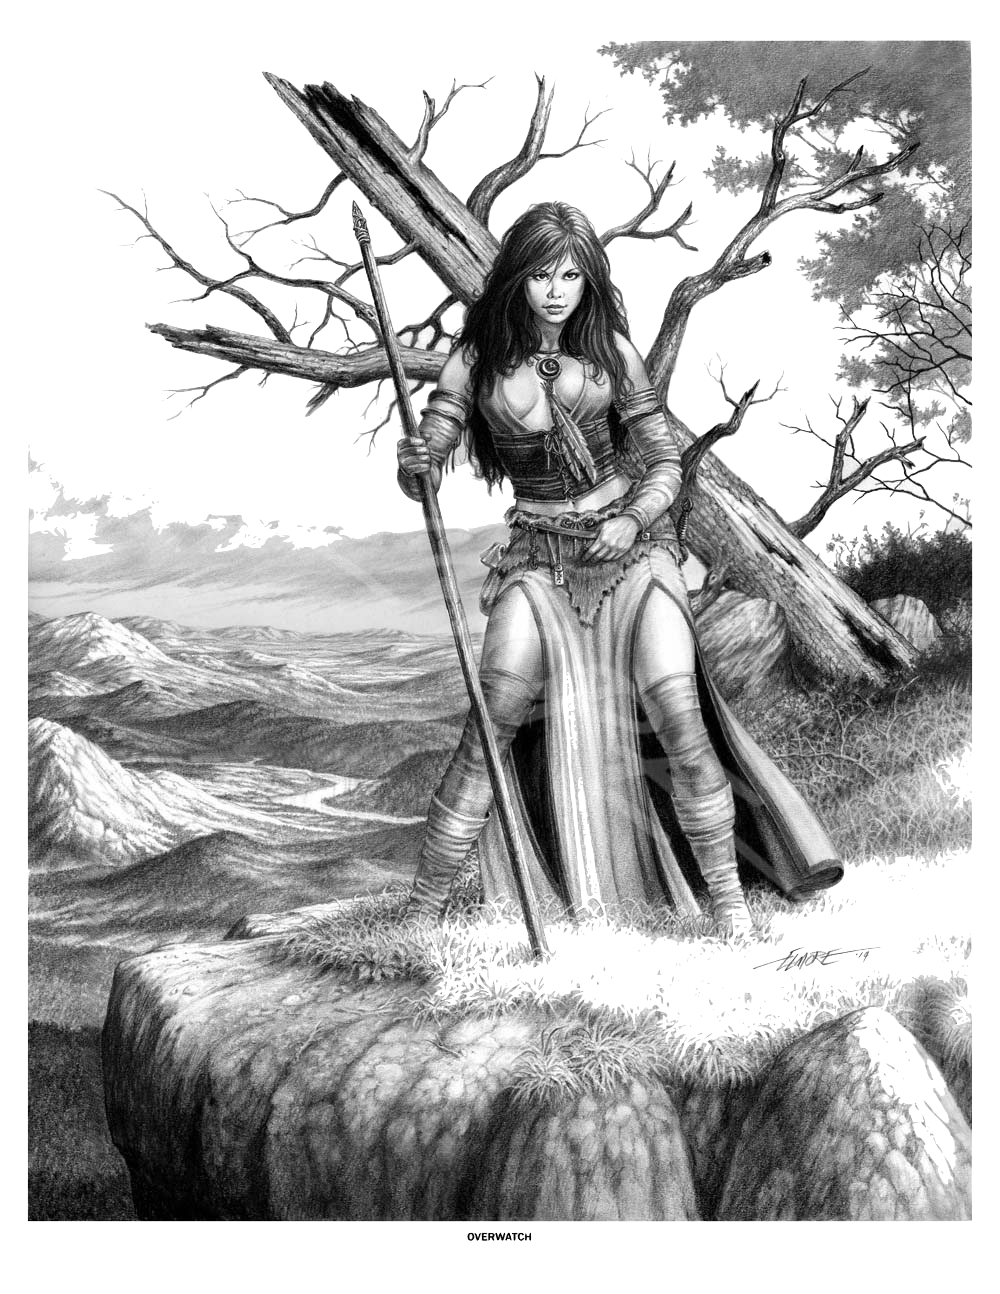
\includegraphics[width=\textwidth]{img/druid-2.png}
\end{Figure}
    
\end{multicols*}


\clearpage

\begin{table}[ht!]
\begin{small}
\rowcolors{2}{}{commentgreen}
\begin{center}
\begin{tabular}{ll}
\multicolumn{2}{l}{\parbox[l][0.6cm][c]{15cm}{\textbf{Arcanist Metamagic}}} 
\\
\hline 
\textbf{Name} & \parbox[l][0.6cm][c]{15cm}{\textbf{Description}}
\\ 
Air & \parbox[l][2.8cm][c]{15cm}{
You can spend one mana point to create an almost invisible sphere of wind and hovering leaves. The totem emits strong winds causing disadvantage in the first ranged attacks against a creature within 10 feet of the totem. Including itself. This effect activates only once per creature per round.
\\
This totem can fly in any direction. 
}
\\ 
Earth & \parbox[l][2cm][c]{15cm}{
You can spend one mana point to create an orb of dust, rocks, and gravel as a bonus action. The totem emits a burst of positive energy that grants itself and up to three creatures of your choice within 10 feet of it a number of temporary hit points equal to you mana die. The dust barrier protects the creature from natural heat.
}
\\
Fire & \parbox[l][2cm][c]{15cm}{
You can spend one mana point to create a sphere of flames and cinder. The totem must hover directly 5 feet above a create. The warm flames protect the creature from natural cold. Once per round, whenever the protected creature takes melee damage, the sphere rebukes with flames. The attacking creature takes your mana die fire damage.
}
\\ 
Water & \parbox[l][2.2cm][c]{15cm}{
You can spend one mana point to create an orb of water and ice. The water sphere fires ice javelins upon your command. 
Make a ranged spell attack, originating from the water sphere, at one creature or object within 120 feet of it. On a hit, the target takes your mana die damage + your spellcasting ability modifier ice damage.
}
\\
\hline
\end{tabular}
\end{center}
\end{small}
\end{table}    


\begin{multicols*}{2}
\begin{Figure}
\centering
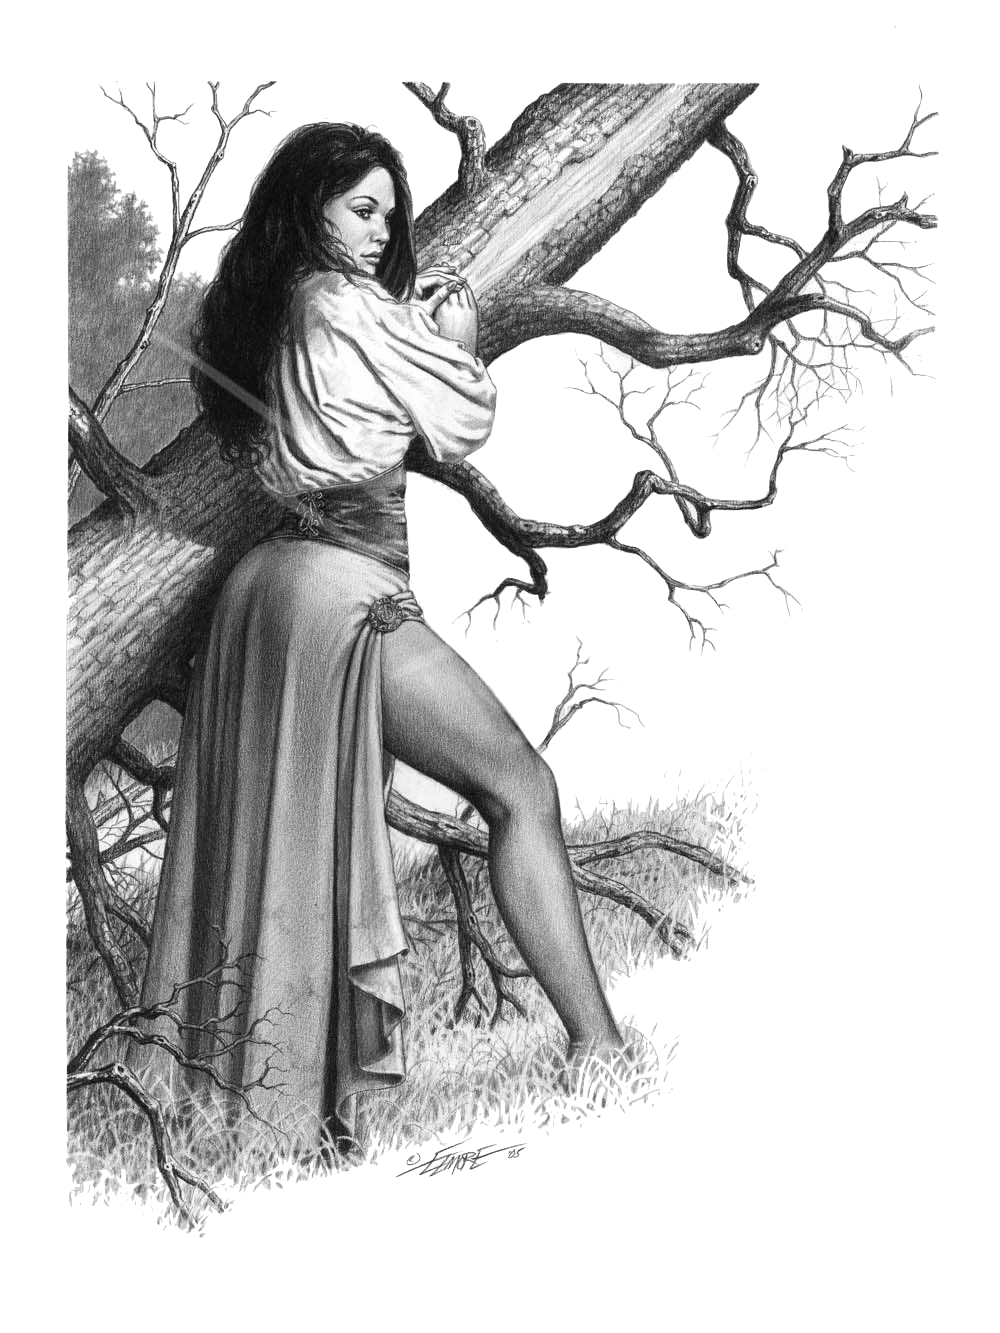
\includegraphics[width=\textwidth]{img/bard.png}
\end{Figure}
    
\end{multicols*}

        